%%%
%% Testing :: Functional Testing
%%%
\section{Functional Testing}
\label{sec:functional_testing}

The purpose of the functional testing is to take all the requirements apart from
the non-functional requirements and determine whether they have been achieved
from the final system. 

This section will take all the requirements from the Functional Requirements and
Usability Requirements found within the MoSCoW analysis section and will provide
evidence of the requirements being fulfilled. If the requirements have not been 
implemented, an explanation will be delivered as to the reasons why.


%%%
%% Testing :: Functional Testing :: Functional Requirements
%%%
\subsection{Functional Requirements}
\label{sub:test_func_func}


\paragraph{Retrieve and process cryptic clues and output possible solutions}

A website and a web service have been implemented. The website allows the input
of cryptic clues and clue details from the user which are then passed to the web
service  for all the solver algorithms to find potential solutions. These
potential solutions are then  sent back to the website to be displayed for the
user.

\begin{figure}[H]
	\centering
	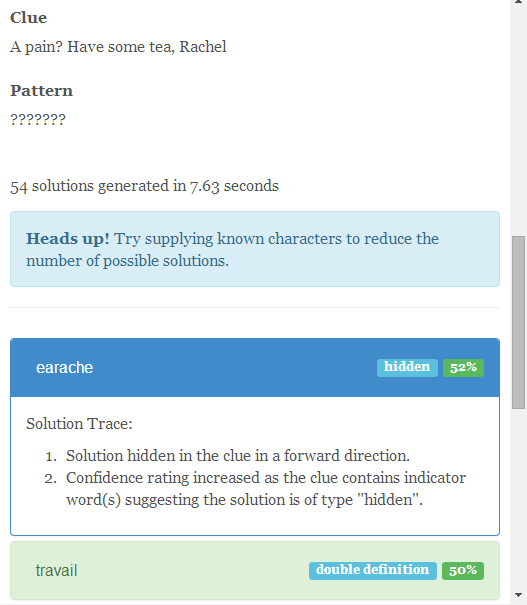
\includegraphics[keepaspectratio=true,scale=0.4]{evidence/retrieve.png}
	\caption{Cryptic clue with results retrieved from web service}
\end{figure}

{\bf Overall:} Fully Implemented


\paragraph{Obtain characteristics of the clue's solution (e.g. number of words,
word lengths and known letters) and match these against possible solutions}

A web interface has been implemented with the necessary controls for the user
to successfully implement the required and optional information associated with
a cryptic clue.

\begin{figure}[H]
	\centering
	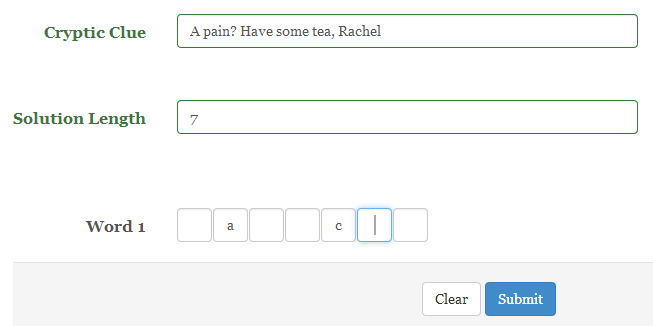
\includegraphics[keepaspectratio=true]{evidence/obtain.png}
	\caption{Input fields for obtaining characteristics of a cryptic clue}
\end{figure}

{\bf Overall:} Fully Implemented


\paragraph{Provide a web interface for users to interact with the system}

A web interface has been implemented to allow users to interact with the web
service.

\begin{figure}[H]
	\centering
	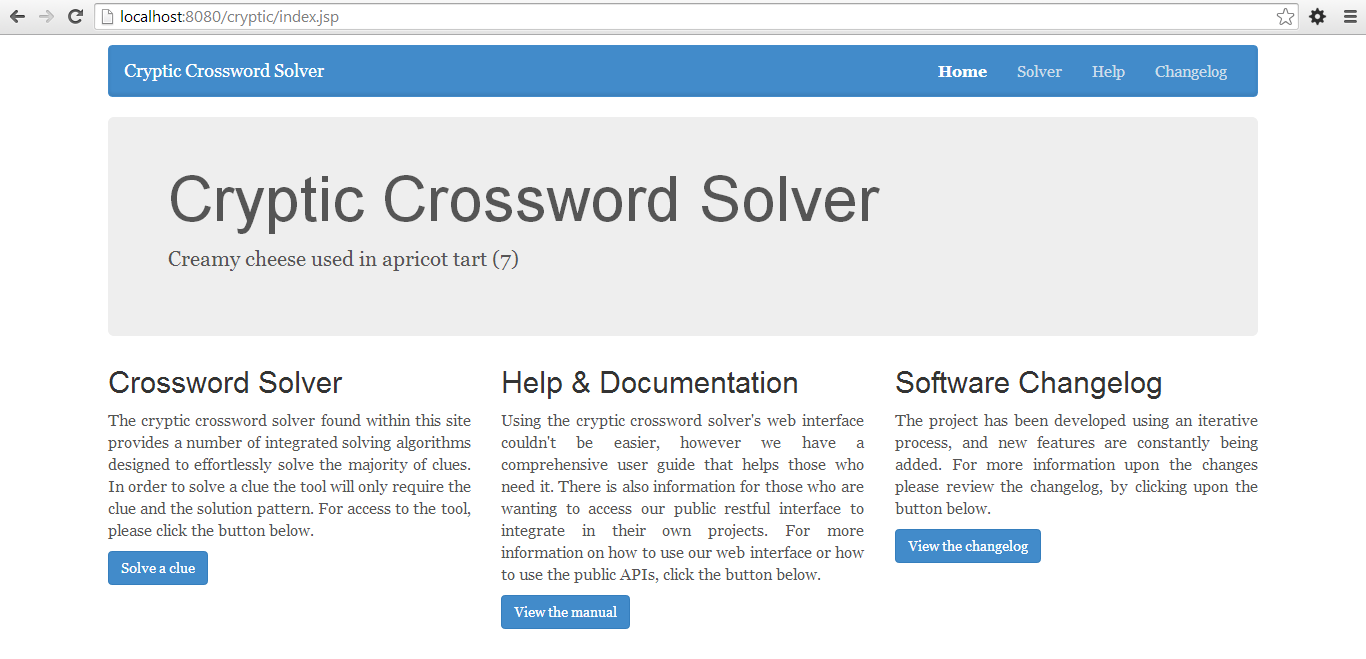
\includegraphics[keepaspectratio=true,scale=0.4]{evidence/scrolling.png}
	\caption{Web page in full screen browser window}
\end{figure}

{\bf Overall:} Fully Implemented


\paragraph{Provide a mobile-friendly interface for users to interact with the
system}

The web interface that has been implemented has been implemented in such a way
that it resizes with the browser window. Therefore, even though it was not made
for  mobile devices it has a mobile-friendly interface with as limited scrolling
as possible.

\begin{figure}[H]
	\centering
	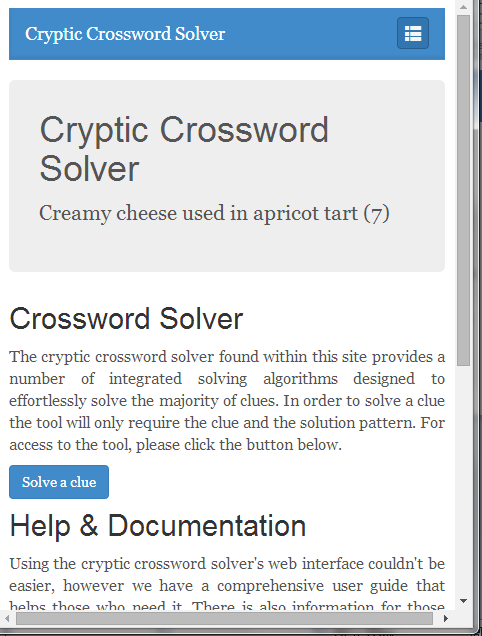
\includegraphics[keepaspectratio=true,scale=0.5]{evidence/scrolling1.png}
	\caption{Web page in resized browser window}
\end{figure}

{\bf Overall:} Partially Implemented


\paragraph{Store clues and their corresponding solutions for future retrieval,
including the clue type and solution length}

The database used within the project is purely for testing purposes. It was
decided during the implementation stage that a database to store clues along
with their details for the use of the web service before passing the clue to
the solvers was not necessary because it may not be entirely beneficial. To
store exact clues  in the database would mean the user would have to input the
exact same  clue (wording and punctuation) for this to be beneficial.

{\bf Overall:} Not Implemented


\paragraph{Take feedback from a user on a solution's accuracy and use this to
rank solutions for a given clue}

As a database has not been implemented for the uses other than testing, this
requirement was not possible.

{\bf Overall:} Not Implemented


\paragraph{Relay the process (solution trace) followed to arrive at a proposed
solution to the user}

Whilst the solvers are finding potential solutions, each solution builds up its
own trace. This trace holds important aspects of how the associated solution
has been found. These traces are then passed back to the web page to be
displayed  with the solution for the user.

\begin{figure}[H]
	\centering
	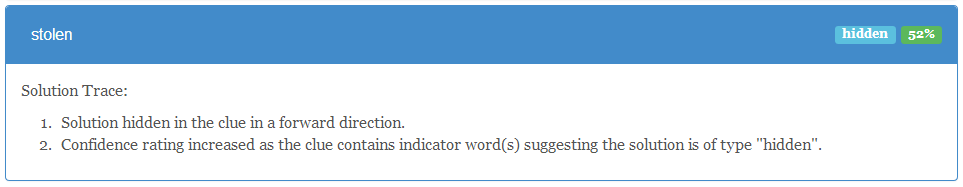
\includegraphics[keepaspectratio=true,scale=0.5]{evidence/trace1.png}
	\caption{Trace for solution `stolen' with clue; `Among library books to lend 
	and not returned', with solution; `stolen'}
\end{figure}

\begin{figure}[H]
	\centering
	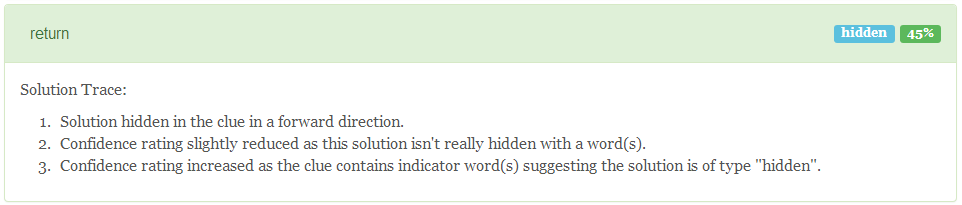
\includegraphics[keepaspectratio=true,scale=0.5]{evidence/trace2.png}
	\caption{Trace for solution `return' with clue; `Among library books to lend 
	and not returned', with solution; `stolen'}
	\label{fig:decCon}
\end{figure}


{\bf Overall:} Fully Implemented


\paragraph{Holistically determine a confidence score for each proposed
solution, and relay this to the user}

The confidence score is increased if indicator words or synonyms that match clue
words are found. Confidence scores can also be decreased, as shown in Figure
\ref{fig:decCon}.

\begin{figure}[H]
	\centering
	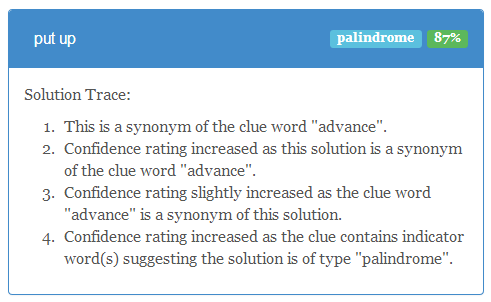
\includegraphics[keepaspectratio=true]{evidence/confidence.png}
	\caption{A solution returned with a confidence score displayed of 87\% for the
	clue; `Advance in either direction'}
\end{figure}

{\bf Overall:} Fully Implemented


\paragraph{Document and store the process (solution trace) followed to solve a
given clue}

As a database has not been implemented for the uses other than testing, this
requirement was not possible.

{\bf Overall:} Not Implemented


\paragraph{Solve clues which take cues from the clue's orientation or clue
number in the crossword}

As the chance of this occurring is rare, it was not seen as beneficial to
implement.

{\bf Overall:} Not Implemented


\paragraph{Provide real-time feedback of the processes being followed by the
application in an attempt to calculate the correct solution}

{\bf Overall:} Not Implemented


\paragraph{Take annotations provided by the user of the known aspects of a clue,
such as the definition word(s), fodder or indicator word(s)}

Although this would have been a beneficial requirement to implement for the
project, unfortunately development time was limited. This could have been
integrated with the Categoriser to increase confidence scores and possibly
bring in the functionality to pass the clue to specific solvers rather than all
of them.

{\bf Overall:} Not Implemented


\paragraph{Store a clue's orientation and clue number in the database}

As a database has not been implemented for the uses other than testing, this
requirement was not possible.

{\bf Overall:} Not Implemented


\paragraph{Use stored data to generate complete cryptic crosswords}

As a database has not been implemented for the uses other than testing,  this
requirement was not possible. It was also stated as a `Not' requirement  within
the MoSCoW analysis.

{\bf Overall:} Not Implemented


\paragraph{Provide a personalised service, including a history of a user's
interactions with the system}

As a database has not been implemented for the uses other than testing,  this
requirement was not possible. It was also stated as a `Not' requirement  within
the MoSCoW analysis.

{\bf Overall:} Not Implemented


%%%
%% Testing :: Functional Testing :: Usability Requirements
%%%
\subsection{Usability Requirements}
\label{sub:test_func_usability}


\paragraph{Provide a text field for the user to input the cryptic clue to be}

A text field has been added to the interface to allow the user to enter a 
cryptic clue. 

\begin{figure}[H]
	\centering
	 
\includegraphics[keepaspectratio=true]{evidence/enterclue.png}
	\caption{Text field to enter clue}
\end{figure}

{\bf Overall:} Fully Implemented


\paragraph{Provide a drop-down box allowing the user to input the number of
words in the solution, with an initial upper- limit of 10 words}

A text field has been provided instead of a drop-down box which allows the user
to input the number of words as well as the length of the words. The limit on
the amount of words input by the user has not been implemented, however the
user  can only input words of length up to fifteen. This is because a
traditional cryptic  crossword has a typical size of 15x15.

\begin{figure}[H]
	\centering
	
\includegraphics[keepaspectratio=true]{evidence/dropdown1.png}
	\caption{Attempting to enter a length of sixteen - the red colour signifies it
	is invalid}
\end{figure}

\begin{figure}[H]
	\centering
	
\includegraphics[keepaspectratio=true]{evidence/dropdown2.png}
	\caption{Attempting to enter two words of length fifteen - the green colour 
	signifies it is valid}
\end{figure}

\begin{figure}[H]
	\centering
	
\includegraphics[keepaspectratio=true]{evidence/dropdown3.png}
	\caption{Attempting to enter three words of valid length with a space and a 
	hyphen - the green colour signifies it is valid}
\end{figure}

{\bf Overall:} Alternatively Implemented


\paragraph{Dynamically provide individual text boxes for each word of the
solution, which allow the length of the words to be specified. Also provide
check-boxes between these text- boxes to define whether they are separated by a
space or a hyphen}

See `Provide a drop-down box allowing the user to input the number of words in
the solution, with an initial upper- limit of 10 words'.

{\bf Overall:} Alternatively Implemented


\paragraph{Dynamically provide text boxes to represent each character of each
word of the solution, allowing the user to input any known characters}

Text boxes are dynamically created depending on the values input into the
`Solution Length' field.

\begin{figure}[H]
	\centering
	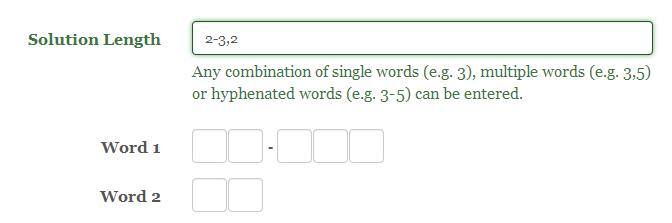
\includegraphics[keepaspectratio=true,scale=0.9]{evidence/dynamicboxes.png}
	\caption{Boxes that have been generated for a solution with the configuration;
	2-3,2}
\end{figure}

{\bf Overall:} Fully Implemented


\paragraph{Provide a table of results which allow the user the to view the
possible solutions}

When the results are returned to the user, they are displayed within a table
underneath the fields containing the users input.

\begin{figure}[H]
	\centering
	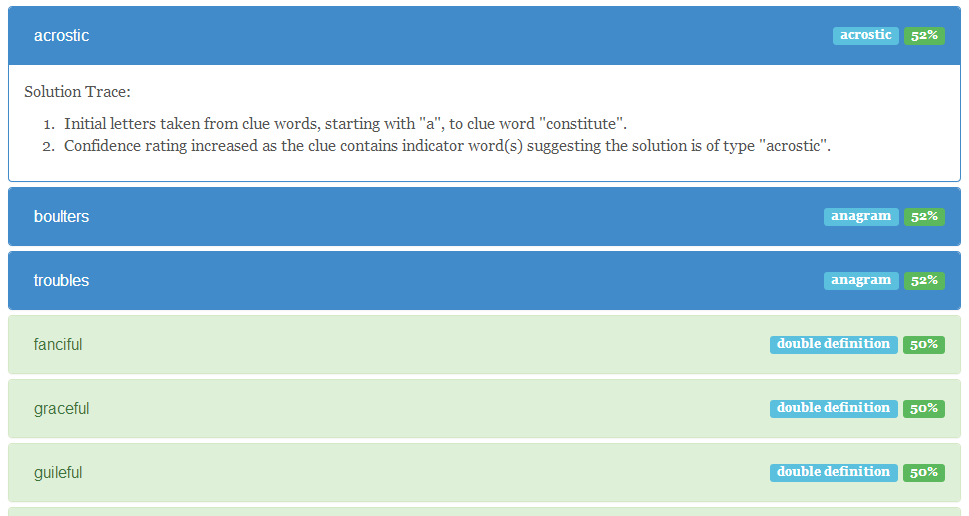
\includegraphics[keepaspectratio=true,scale=0.6]{evidence/listsolutions.png}
	\caption{Results displayed for the clue; `A clever rhyme or subtle teaser I constitute'}
\end{figure}

{\bf Overall:}: Fully Implemented


\paragraph{Alert the user to required fields with red asterisks}    

A design decision was made to change the colour of the label text  and the
outline of the text box if the user clicks `Submit' without filling in  required
fields.

\begin{figure}[H]
	\centering
	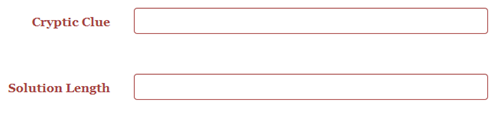
\includegraphics[keepaspectratio=true]{evidence/alert1.png}
	\caption{If the user submits without filling in either required fields}
\end{figure}

\begin{figure}[H]
	\centering
	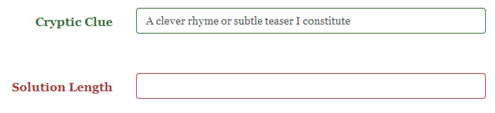
\includegraphics[keepaspectratio=true]{evidence/alert2.png}
	\caption{If the user submits without filling in the length of the solution}
\end{figure}

\begin{figure}[H]
	\centering
	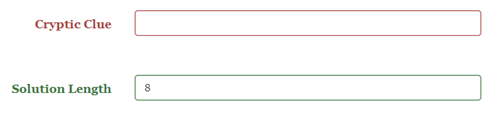
\includegraphics[keepaspectratio=true]{evidence/alert3.png}
	\caption{If the user submits without filling in the clue field}
\end{figure}

{\bf Overall:} Alternatively Implemented


\paragraph{Have a consistent layout avoid unnecessary scrolling}

All pages within the website have the same colour scheme and fonts  with an
additional consistency with menu items and bars. The web page  has also been
implemented to resize to the browser window. This means  there is no scrolling
for full screen browser windows and limited horizontal  scrolling for smaller
browser windows as the controls are moved into a linear  position.

\begin{figure}[H]
	\centering
	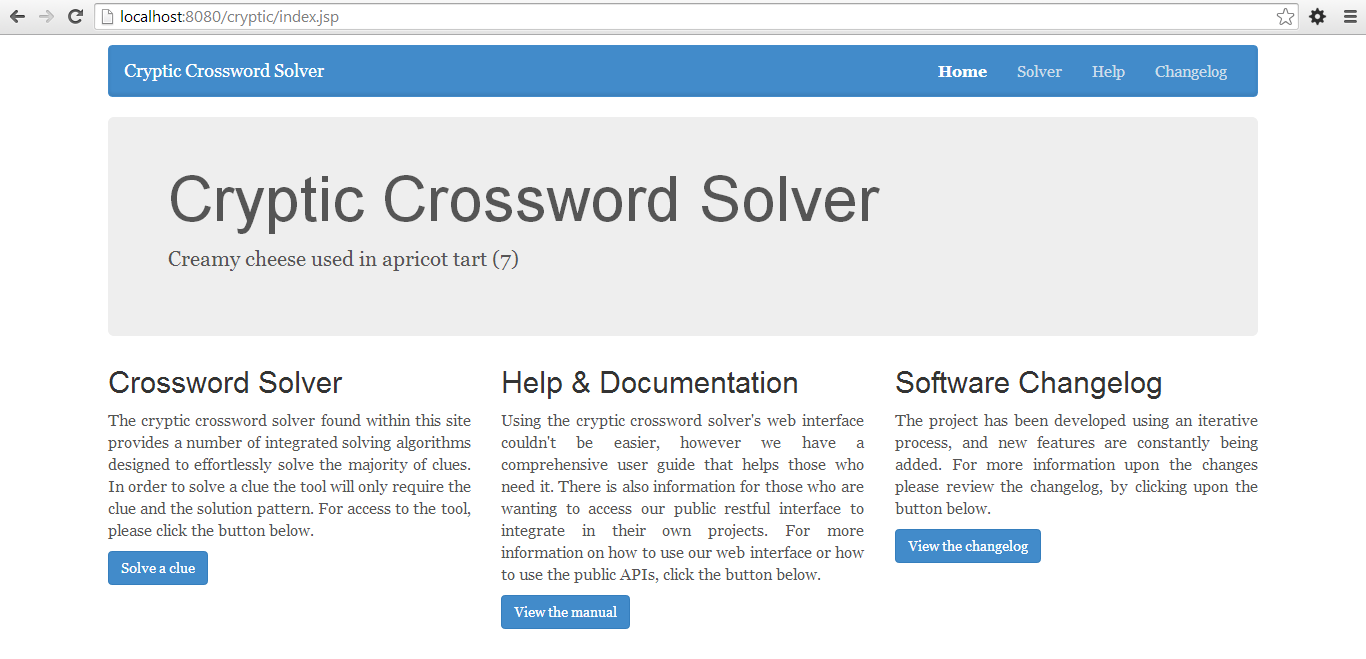
\includegraphics[keepaspectratio=true,scale=0.4]{evidence/scrolling.png}
	\caption{Web page in full screen browser window}
\end{figure}

\begin{figure}[H]
	\centering
	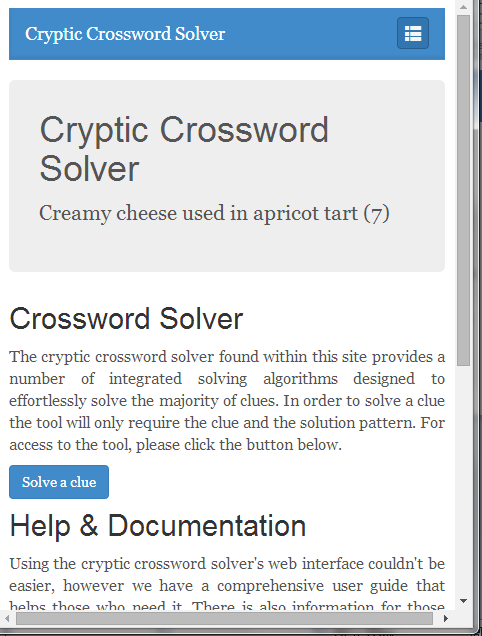
\includegraphics[keepaspectratio=true,scale=0.5]{evidence/scrolling1.png}
	\caption{Web page in resized browser window}
\end{figure}

{\bf Overall:} Fully Implemented


\paragraph{Alert the user to invalid input through validation checks with error
messages}
     
When the user clicks `Submit' without completing the required fields the
styling of the label and text fields change colour to red and the page does not
proceed to pass invalid data to the back end code.

See `Alert the user to required fields with red asterisks' for evidence'.

{\bf Overall:} Alternatively Implemented 


\paragraph{Provide a confidence rating in the table of possible solutions}

The confidence rating calculated whilst retrieving possible solutions is 
displayed alongside the solution.

\begin{figure}[H]
	\centering
	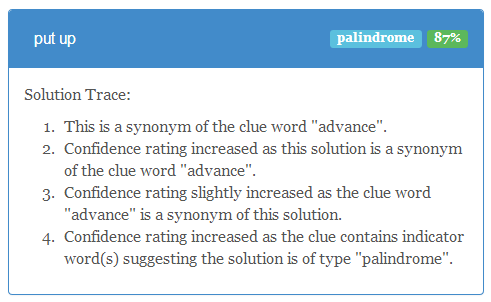
\includegraphics[keepaspectratio=true]{evidence/confidence.png}
	\caption{Confidence ratings displayed with the solutions returned}
\end{figure}

{\bf Overall:} Fully Implemented


\paragraph{Allow the user to select a proposed solution in the corresponding
table and mark this as correct}

{\bf Overall:} Not Implemented


\paragraph{Display help buttons to indicate to the user the purpose and use of
each control}

Instead of implementing buttons to display help for each of the controls on the
web page,  a user manual has been created which can be accessed through the menu
bar. This explains  the web page functionality as well as some additional
information on the web service.

\begin{figure}[H]
	\centering
	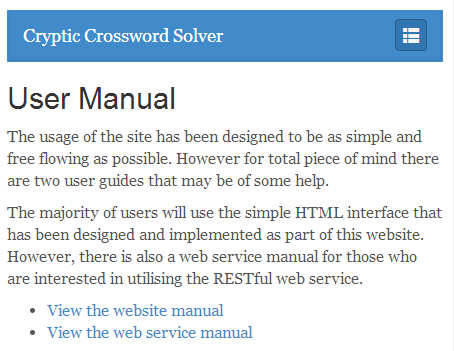
\includegraphics[keepaspectratio=true]{evidence/manual.png}
	\caption{Introduction to the user manual}
\end{figure}

{\bf Overall:} Alternatively Implemented


\paragraph{Provide a button to submit the user input to the application for
processing}

A submit button has been provided for the user to click when they have input
the clue itself and the clues length.

\begin{figure}[H]
	\centering
	
\includegraphics[keepaspectratio=true]{evidence/submit.png}
	\caption{Submit button for user to click}
\end{figure}

{\bf Overall:} Fully Implemented


\paragraph{Provide a group of radio buttons for the user to select the clue's
orientation in its containing crossword}

There has been no functionality implemented to use the clue's orientation
within the solver algorithms, therefore it was unnecessary to implement radio
buttons for the user to select the orientation of the clue.

{\bf Overall:} Not Implemented


\paragraph{Provide a text box to input the clue's number within its containing
crossword}

There has been no functionality implemented to use the clue's grid number
within the solver algorithms, therefore it was unnecessary to implement a text
box for the user to input the grid number of the clue.
 
{\bf Overall:} Not Implemented


\paragraph{Provide mechanisms to accommodate for users with difficulties, such
as colour-blindness or poor eyesight}
    
There has been no specific functionality implemented to accommodate for  users
with difficulties. However, the user can disable CSS on their browser  to view
the web page with no styling.

{\bf Overall:} Not Implemented
